% ============================================================
% Question Bank: ch01-03 Finding the Constant of Proportionality
% Topic Title: Finding the Constant of Proportionality
% CCSS: 7.RP.A.2b
% Questions: 27 (15 MC + 6 SA + 6 Graphical)
% ============================================================

% --- Multiple Choice Questions (15) ---

\begin{practiceQuestion}{1-3-q01}{mc}
\begin{questionText}
The table below shows a proportional relationship between the number of gallons of gas and the cost.

\begin{center}
\begin{tabular}{|c|c|}
\hline
\textbf{Gallons} & \textbf{Cost (\$)} \\
\hline
$3$ & $\$10.50$ \\
$5$ & $\$17.50$ \\
$8$ & $\$28.00$ \\
\hline
\end{tabular}
\end{center}

What is the constant of proportionality?
\end{questionText}
\choiceA{$\$2.50$}
\choiceB{$\$3.00$}
\choiceC{$\$3.50$}
\choiceD{$\$7.00$}
\correctAnswer{C}
\explanation{The constant of proportionality is $k = \frac{y}{x}$. Divide cost by gallons: $\frac{10.50}{3} = 3.50$. Check: $\frac{17.50}{5} = 3.50$ and $\frac{28.00}{8} = 3.50$. So $k = 3.50$.}
\end{practiceQuestion}

\begin{practiceQuestion}{1-3-q02}{mc}
\begin{questionText}
A proportional relationship passes through the point $(8, 20)$. What is the constant of proportionality?
\end{questionText}
\choiceA{$k = 12$}
\choiceB{$k = 0.4$}
\choiceC{$k = 2.5$}
\choiceD{$k = 160$}
\correctAnswer{C}
\explanation{For a proportional relationship, $k = \frac{y}{x} = \frac{20}{8} = 2.5$. This means $y$ increases by $2.5$ for every $1$ unit of $x$.}
\end{practiceQuestion}

\begin{practiceQuestion}{1-3-q03}{mc}
\begin{questionText}
A bakery sells muffins at a constant price. Four muffins cost $\$6.00$ and ten muffins cost $\$15.00$. What is $k$, the cost per muffin?
\end{questionText}
\choiceA{$k = 1.25$}
\choiceB{$k = 1.50$}
\choiceC{$k = 2.00$}
\choiceD{$k = 6.00$}
\correctAnswer{B}
\explanation{Divide cost by quantity: $6.00 \div 4 = 1.50$ and $15.00 \div 10 = 1.50$. The constant of proportionality is $k = \$1.50$ per muffin.}
\end{practiceQuestion}

\begin{practiceQuestion}{1-3-q04}{mc}
\begin{questionText}
On a proportional graph, the $y$-value when $x = 1$ is $7$. What is the constant of proportionality?
\end{questionText}
\choiceA{$k = 0$}
\choiceB{$k = 1$}
\choiceC{$k = 7$}
\choiceD{$k = \frac{1}{7}$}
\correctAnswer{C}
\explanation{On a proportional graph, the point $(1, r)$ gives the unit rate directly. Since $y = 7$ when $x = 1$, the constant of proportionality is $k = 7$.}
\end{practiceQuestion}

\begin{practiceQuestion}{1-3-q05}{mc}
\begin{questionText}
The table below shows the number of pages a student reads over time.

\begin{center}
\begin{tabular}{|c|c|}
\hline
\textbf{Minutes} & \textbf{Pages} \\
\hline
$10$ & $8$ \\
$25$ & $20$ \\
$40$ & $32$ \\
\hline
\end{tabular}
\end{center}

What does the constant of proportionality represent in this context?
\end{questionText}
\choiceA{The total number of pages read}
\choiceB{The number of pages read per minute}
\choiceC{The number of minutes per page}
\choiceD{The difference between pages and minutes}
\correctAnswer{B}
\explanation{The constant of proportionality $k = \frac{8}{10} = 0.8$ pages per minute. It represents the number of pages the student reads for every $1$ minute of reading time.}
\end{practiceQuestion}

\begin{practiceQuestion}{1-3-q06}{mc}
\begin{questionText}
A recipe uses cups of flour ($y$) proportionally to the number of servings ($x$). The table shows:

\begin{center}
\begin{tabular}{|c|c|}
\hline
\textbf{Servings} & \textbf{Flour (cups)} \\
\hline
$6$ & $4.5$ \\
$10$ & $?$ \\
\hline
\end{tabular}
\end{center}

How many cups of flour are needed for $10$ servings?
\end{questionText}
\choiceA{$5.0$}
\choiceB{$6.5$}
\choiceC{$7.5$}
\choiceD{$10.5$}
\correctAnswer{C}
\explanation{Find $k$: $\frac{4.5}{6} = 0.75$ cups per serving. Multiply: $0.75 \times 10 = 7.5$ cups of flour for $10$ servings.}
\end{practiceQuestion}

\begin{practiceQuestion}{1-3-q07}{mc}
\begin{questionText}
Which of the following points on a proportional graph would give a constant of proportionality of $\frac{3}{4}$?
\end{questionText}
\choiceA{$(3, 4)$}
\choiceB{$(4, 3)$}
\choiceC{$(8, 6)$}
\choiceD{Both B and C}
\correctAnswer{D}
\explanation{Check each: $(4, 3)$ gives $k = \frac{3}{4}$ and $(8, 6)$ gives $k = \frac{6}{8} = \frac{3}{4}$. Both produce the same constant of proportionality. $(3, 4)$ gives $k = \frac{4}{3}$, which is the reciprocal.}
\end{practiceQuestion}

\begin{practiceQuestion}{1-3-q08}{mc}
\begin{questionText}
A car travels at a constant speed. In $\frac{1}{2}$ hour it covers $32$ miles. What is the constant of proportionality in miles per hour?
\end{questionText}
\choiceA{$16$}
\choiceB{$32$}
\choiceC{$48$}
\choiceD{$64$}
\correctAnswer{D}
\explanation{Divide miles by hours: $k = \frac{32}{\frac{1}{2}} = 32 \times 2 = 64$ miles per hour. This is the unit rate --- the car travels $64$ miles in $1$ hour.}
\end{practiceQuestion}

\begin{practiceQuestion}{1-3-q09}{mc}
\begin{questionText}
Marcus says the constant of proportionality in the table below is $5$ because "$y$ increases by $5$ each time."

\begin{center}
\begin{tabular}{|c|c|}
\hline
$x$ & $y$ \\
\hline
$2$ & $5$ \\
$4$ & $10$ \\
$6$ & $15$ \\
\hline
\end{tabular}
\end{center}

What is Marcus's error?
\end{questionText}
\choiceA{He should have added $x$ and $y$.}
\choiceB{He found the difference between $y$-values instead of dividing $y$ by $x$.}
\choiceC{He forgot to simplify the fraction.}
\choiceD{There is no error; Marcus is correct.}
\correctAnswer{B}
\explanation{The constant of proportionality is $k = \frac{y}{x}$, not the difference between consecutive $y$-values. Here $k = \frac{5}{2} = 2.5$. Marcus confused the constant change in $y$ with the constant ratio $\frac{y}{x}$.}
\end{practiceQuestion}

\begin{practiceQuestion}{1-3-q10}{mc}
\begin{questionText}
A proportional graph passes through $(5, 12.5)$ and $(10, 25)$. What is $k$?
\end{questionText}
\choiceA{$k = 0.4$}
\choiceB{$k = 2$}
\choiceC{$k = 2.5$}
\choiceD{$k = 7.5$}
\correctAnswer{C}
\explanation{Use either point: $k = \frac{12.5}{5} = 2.5$ or $k = \frac{25}{10} = 2.5$. The constant of proportionality is $2.5$.}
\end{practiceQuestion}

\begin{practiceQuestion}{1-3-q11}{mc}
\begin{questionText}
A machine makes $36$ widgets in $4$ minutes. Another machine makes $54$ widgets in $6$ minutes. Which statement is true?
\end{questionText}
\choiceA{The first machine is faster because $36 > 54 \div 2$.}
\choiceB{The second machine is faster because $54 > 36$.}
\choiceC{Both machines have the same constant of proportionality.}
\choiceD{The first machine has a greater constant of proportionality.}
\correctAnswer{C}
\explanation{Find each constant: Machine 1: $k = \frac{36}{4} = 9$. Machine 2: $k = \frac{54}{6} = 9$. Both produce $9$ widgets per minute, so the constants are equal.}
\end{practiceQuestion}

\begin{practiceQuestion}{1-3-q12}{mc}
\begin{questionText}
In a proportional relationship, $k = 4.5$. What is the value of $y$ when $x = 12$?
\end{questionText}
\choiceA{$y = 16.5$}
\choiceB{$y = 48$}
\choiceC{$y = 54$}
\choiceD{$y = 2\frac{2}{3}$}
\correctAnswer{C}
\explanation{In a proportional relationship $y = kx$. Substitute: $y = 4.5 \times 12 = 54$.}
\end{practiceQuestion}

\begin{practiceQuestion}{1-3-q13}{mc}
\begin{questionText}
The table below represents a proportional relationship. What is the missing value?

\begin{center}
\begin{tabular}{|c|c|}
\hline
$x$ & $y$ \\
\hline
$3$ & $7.5$ \\
$7$ & $?$ \\
$12$ & $30$ \\
\hline
\end{tabular}
\end{center}
\end{questionText}
\choiceA{$10.5$}
\choiceB{$14$}
\choiceC{$17.5$}
\choiceD{$21$}
\correctAnswer{C}
\explanation{Find $k$ from the first row: $k = \frac{7.5}{3} = 2.5$. Then $y = 2.5 \times 7 = 17.5$. Check: $2.5 \times 12 = 30$ \checkmark.}
\end{practiceQuestion}

\begin{practiceQuestion}{1-3-q14}{mc}
\begin{questionText}
A bike rental charges by the hour. The table shows the cost.

\begin{center}
\begin{tabular}{|c|c|}
\hline
\textbf{Hours} & \textbf{Cost (\$)} \\
\hline
$\frac{1}{2}$ & $\$4.50$ \\
$1$ & $\$9.00$ \\
$3$ & $\$27.00$ \\
\hline
\end{tabular}
\end{center}

What is the constant of proportionality, and what does it mean?
\end{questionText}
\choiceA{$k = 4.50$; it costs $\$4.50$ per half hour}
\choiceB{$k = 9$; it costs $\$9.00$ per hour}
\choiceC{$k = 27$; the total cost is $\$27$}
\choiceD{$k = 3$; the rental is for $3$ hours}
\correctAnswer{B}
\explanation{Divide cost by hours: $\frac{4.50}{0.5} = 9$, $\frac{9}{1} = 9$, $\frac{27}{3} = 9$. The constant of proportionality is $k = 9$, meaning the rental costs $\$9$ per hour.}
\end{practiceQuestion}

\begin{practiceQuestion}{1-3-q15}{mc}
\begin{questionText}
On a proportional graph, Line $A$ passes through $(2, 8)$ and Line $B$ passes through $(2, 5)$. Both pass through the origin. Which line has the greater constant of proportionality?
\end{questionText}
\choiceA{Line $A$, because $k_A = 4 > k_B = 2.5$}
\choiceB{Line $B$, because $k_B = 5 > k_A = 8$}
\choiceC{They are equal because both pass through $x = 2$.}
\choiceD{Line $B$, because $5$ is a whole number}
\correctAnswer{A}
\explanation{Line $A$: $k = \frac{8}{2} = 4$. Line $B$: $k = \frac{5}{2} = 2.5$. Since $4 > 2.5$, Line $A$ has the greater constant of proportionality and is the steeper line.}
\end{practiceQuestion}

% --- Short Answer Questions (6) ---

\begin{practiceQuestion}{1-3-q16}{sa}
\begin{questionText}
A photocopy machine prints $45$ copies in $3$ minutes at a constant rate. What is the constant of proportionality in copies per minute?
\end{questionText}
\correctAnswer{$15$}
\explanation{Divide copies by minutes: $k = \frac{45}{3} = 15$ copies per minute. The machine prints $15$ copies every minute.}
\end{practiceQuestion}

\begin{practiceQuestion}{1-3-q17}{sa}
\begin{questionText}
In a proportional relationship, $y = 56$ when $x = 8$. Find the value of $x$ when $y = 91$.
\end{questionText}
\correctAnswer{$13$}
\explanation{Find $k$: $k = \frac{56}{8} = 7$. Then use $y = 7x$ to solve: $91 = 7x$, so $x = \frac{91}{7} = 13$.}
\end{practiceQuestion}

\begin{practiceQuestion}{1-3-q18}{sa}
\begin{questionText}
A car's odometer shows it traveled $195$ miles using $6$ gallons of gas. What is the constant of proportionality in miles per gallon?
\end{questionText}
\correctAnswer{$32.5$}
\explanation{Divide miles by gallons: $k = \frac{195}{6} = 32.5$ miles per gallon. The car travels $32.5$ miles on each gallon of gas.}
\end{practiceQuestion}

\begin{practiceQuestion}{1-3-q19}{sa}
\begin{questionText}
A proportional relationship has $k = \frac{2}{3}$. When $x = 15$, what is $y$?
\end{questionText}
\correctAnswer{$10$}
\explanation{Use $y = kx$: $y = \frac{2}{3} \times 15 = \frac{30}{3} = 10$.}
\end{practiceQuestion}

\begin{practiceQuestion}{1-3-q20}{sa}
\begin{questionText}
The table shows a proportional relationship. Find the missing value.

\begin{center}
\begin{tabular}{|c|c|}
\hline
$x$ & $y$ \\
\hline
$5$ & $8$ \\
$15$ & $?$ \\
\hline
\end{tabular}
\end{center}
\end{questionText}
\correctAnswer{$24$}
\explanation{Find $k$: $k = \frac{8}{5} = 1.6$. Then $y = 1.6 \times 15 = 24$.}
\end{practiceQuestion}

\begin{practiceQuestion}{1-3-q21}{sa}
\begin{questionText}
A fruit punch recipe mixes juice and water proportionally. If $3$ cups of juice are mixed with $5$ cups of water, how many cups of water are needed for $9$ cups of juice?
\end{questionText}
\correctAnswer{$15$}
\explanation{Find $k$ (water per juice): $k = \frac{5}{3}$. For $9$ cups of juice: $\frac{5}{3} \times 9 = 15$ cups of water.}
\end{practiceQuestion}

% --- Graphical Multiple Choice Questions (3) ---

\begin{practiceQuestion}{1-3-q22}{gmc}
\begin{questionText}
The graph below shows a proportional relationship. What is the constant of proportionality?

\begin{center}
\begin{tikzpicture}[scale=0.55]
  \draw[step=1,gray!20,thin] (0,0) grid (8,8);
  \draw[thick,->] (0,0) -- (8.5,0) node[right]{$x$};
  \draw[thick,->] (0,0) -- (0,8.5) node[above]{$y$};
  \foreach \x in {1,...,8} \draw (\x,0.1) -- (\x,-0.1) node[below]{\tiny \x};
  \foreach \y in {1,...,8} \draw (0.1,\y) -- (-0.1,\y) node[left]{\tiny \y};
  \draw[thick,funBlue] (0,0) -- (8,6);
  \fill[funBlue] (0,0) circle (3pt);
  \fill[funBlue] (4,3) circle (3pt);
  \fill[funBlue] (8,6) circle (3pt);
\end{tikzpicture}
\end{center}
\end{questionText}
\choiceA{$k = \frac{4}{3}$}
\choiceB{$k = \frac{3}{4}$}
\choiceC{$k = 3$}
\choiceD{$k = 4$}
\correctAnswer{B}
\explanation{Read the point $(4, 3)$ from the graph. The constant of proportionality is $k = \frac{y}{x} = \frac{3}{4}$. Check with $(8,6)$: $\frac{6}{8} = \frac{3}{4}$ \checkmark.}
\end{practiceQuestion}

\begin{practiceQuestion}{1-3-q23}{gmc}
\begin{questionText}
The table below shows a proportional relationship. One value is missing.

\begin{center}
\begin{tabular}{|c|c|}
\hline
$x$ & $y$ \\
\hline
$2$ & $9$ \\
$6$ & $27$ \\
$8$ & $?$ \\
\hline
\end{tabular}
\end{center}

What is the missing value of $y$?
\end{questionText}
\choiceA{$32$}
\choiceB{$33$}
\choiceC{$36$}
\choiceD{$40$}
\correctAnswer{C}
\explanation{Find $k$ from the first row: $k = \frac{9}{2} = 4.5$. Then $y = 4.5 \times 8 = 36$. Check: $\frac{27}{6} = 4.5$ \checkmark.}
\end{practiceQuestion}

\begin{practiceQuestion}{1-3-q24}{gmc}
\begin{questionText}
Two proportional lines are graphed on the same axes. Line $P$ passes through $(3, 6)$ and Line $Q$ passes through $(3, 9)$. Both pass through the origin.

\begin{center}
\begin{tikzpicture}[scale=0.45]
  \draw[step=1,gray!20,thin] (0,0) grid (6,12);
  \draw[thick,->] (0,0) -- (6.5,0) node[right]{$x$};
  \draw[thick,->] (0,0) -- (0,12.5) node[above]{$y$};
  \foreach \x in {1,...,6} \draw (\x,0.1) -- (\x,-0.1) node[below]{\tiny \x};
  \foreach \y in {2,4,...,12} \draw (0.1,\y) -- (-0.1,\y) node[left]{\tiny \y};
  \draw[thick,funBlue] (0,0) -- (6,12);
  \draw[thick,funOrange] (0,0) -- (6,12);
  \draw[thick,funBlue] (0,0) -- (5,10);
  \draw[thick,funOrange] (0,0) -- (4,12);
  \fill[funBlue] (3,6) circle (3pt) node[right]{\tiny $P$};
  \fill[funOrange] (3,9) circle (3pt) node[left]{\tiny $Q$};
\end{tikzpicture}
\end{center}

How much greater is $k_Q$ than $k_P$?
\end{questionText}
\choiceA{$1$}
\choiceB{$3$}
\choiceC{$\frac{1}{3}$}
\choiceD{$\frac{3}{2}$}
\correctAnswer{A}
\explanation{$k_P = \frac{6}{3} = 2$ and $k_Q = \frac{9}{3} = 3$. The difference is $3 - 2 = 1$.}
\end{practiceQuestion}

% --- Graphical Short Answer Questions (3) ---

\begin{practiceQuestion}{1-3-q25}{gsa}
\begin{questionText}
The graph below shows the cost of renting roller skates per hour.

\begin{center}
\begin{tikzpicture}[scale=0.5]
  \draw[step=1,gray!20,thin] (0,0) grid (8,10);
  \draw[thick,->] (0,0) -- (8.5,0) node[right]{\small Hours};
  \draw[thick,->] (0,0) -- (0,10.5) node[above]{\small Cost (\$)};
  \foreach \x in {1,...,8} \draw (\x,0.1) -- (\x,-0.1) node[below]{\tiny \x};
  \foreach \y in {1,...,10} \draw (0.1,\y) -- (-0.1,\y) node[left]{\tiny \y};
  \draw[thick,funGreen] (0,0) -- (8,10);
  \fill[funGreen] (0,0) circle (3pt);
  \fill[funGreen] (2,2.5) circle (3pt);
  \fill[funGreen] (4,5) circle (3pt);
  \fill[funGreen] (8,10) circle (3pt);
\end{tikzpicture}
\end{center}

What is the constant of proportionality? Include units.
\end{questionText}
\correctAnswer{$\$1.25$ per hour}
\explanation{Use the point $(4, 5)$: $k = \frac{5}{4} = 1.25$ dollars per hour. Check: $\frac{2.5}{2} = 1.25$ and $\frac{10}{8} = 1.25$ \checkmark.}
\end{practiceQuestion}

\begin{practiceQuestion}{1-3-q26}{gsa}
\begin{questionText}
The double number line below shows a proportional relationship between feet and seconds.

\begin{center}
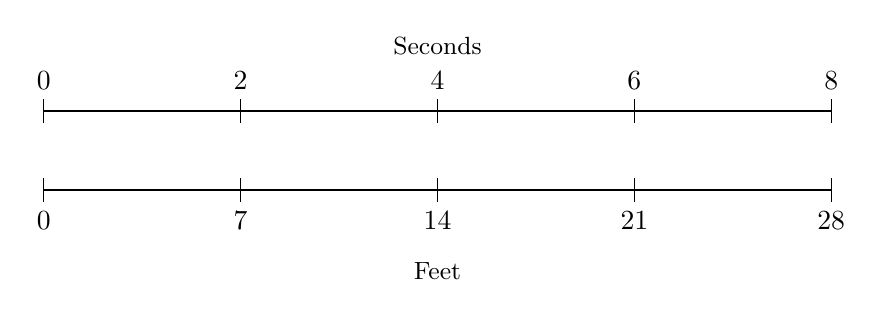
\begin{tikzpicture}[scale=1]
  \draw[thick] (0,0.5) -- (10,0.5);
  \draw[thick] (0,-0.5) -- (10,-0.5);
  \foreach \x/\lab in {0/0, 2.5/2, 5/4, 7.5/6, 10/8}
    \draw (\x,0.35) -- (\x,0.65) node[above]{$\lab$};
  \node[above] at (5,1.1) {\small Seconds};
  \foreach \x/\lab in {0/0, 2.5/7, 5/14, 7.5/21, 10/28}
    \draw (\x,-0.35) -- (\x,-0.65) node[below]{$\lab$};
  \node[below] at (5,-1.3) {\small Feet};
\end{tikzpicture}
\end{center}

What is the constant of proportionality in feet per second?
\end{questionText}
\correctAnswer{$3.5$}
\explanation{Divide feet by seconds from any pair: $\frac{7}{2} = 3.5$, $\frac{14}{4} = 3.5$, $\frac{21}{6} = 3.5$, $\frac{28}{8} = 3.5$. The constant is $3.5$ feet per second.}
\end{practiceQuestion}

\begin{practiceQuestion}{1-3-q27}{gsa}
\begin{questionText}
The table below shows the weight (in ounces) of different numbers of identical bolts.

\begin{center}
\begin{tabular}{|c|c|}
\hline
\textbf{Bolts} & \textbf{Weight (oz)} \\
\hline
$4$ & $3$ \\
$12$ & $9$ \\
$20$ & $15$ \\
$32$ & $?$ \\
\hline
\end{tabular}
\end{center}

Find $k$ and use it to find the missing weight.
\end{questionText}
\correctAnswer{$24$ oz}
\explanation{Find $k$: $\frac{3}{4} = 0.75$ oz per bolt. Check: $\frac{9}{12} = 0.75$ and $\frac{15}{20} = 0.75$ \checkmark. For $32$ bolts: $0.75 \times 32 = 24$ oz.}
\end{practiceQuestion}
